\begin{frame}
	\frametitle{Motivazioni}
			
	\alert{Ispezioni di sicurezza as-a-service} in \alert{reti} o \alert{cloud private}
			
	\begin{itemize}
		\item per ispezionare una cloud pubblica si possono sfruttare
		      gli \alert{hook} messi a disposizione dal cloud provider
		\item in una rete privata \textit{classica} non sono disponibili
		      		      		      
		      \begin{itemize}
		      	\item necessità di passare attraverso \alert{firewall} e \alert{NAT}
		      \end{itemize}
	\end{itemize}
			
\end{frame}

\begin{frame}
	\frametitle{Obiettivi}
	Sviluppare una soluzione che consentisse di:
	\begin{itemize}
		\item fare \alert{ispezioni} in reti e cloud private per
		      valutare lo \alert{stato effettivo} della sicurezza
		\item usando ancora un paradigma \alert{as-a-service}
		\item \alert{configuration-free}
		\item garantire alto livello di sicurezza
	\end{itemize}
\end{frame}

\begin{frame}
	\frametitle{Security assurance e MoonCloud}
	\begin{itemize}
		\item Framework per la \alert{valutazione}
		      ed il \alert{monitoraggio continuo} di servizi
		      cloud
		\item valutazione che certe proprietà (non solo di sicurezza)
		      siano rispettate
		      mediante \alert{raccolta continua di evidenze}
		\item per l'utente finale MoonCloud è offerto \alert{as-a-service}
		      \begin{itemize}
		      	\item inserisce informazioni sul target
		      	\item MoonCloud effettua valutazione
		      	\item mostra risultati
		      \end{itemize}
	\end{itemize}
\end{frame}

\begin{frame}
	\frametitle{Soluzione}
	Utilizzare un collegamento \alert{VPN} (\textit{ponte}) tra MoonCloud e
	la rete da analizzare
		    
	\begin{itemize}
		\item device \alert{Linux} portato nella rete target che fa da VPN client
		\item in MoonCloud i \alert{VPN server}
		\item \alert{OpenVPN} per il collegamento VPN 
		\item \alert{nftables} (successore
		      di \alert{iptables}) per risolvere problemi di configurazione
		      		      		      
	\end{itemize}
		    
	\begin{itemize}
		\item installazione di \alert{VPN non standard}, con numerose problematiche 
	\end{itemize}
\end{frame}

\begin{frame}
	\frametitle{Soluzione (2)}
	\begin{figure}
		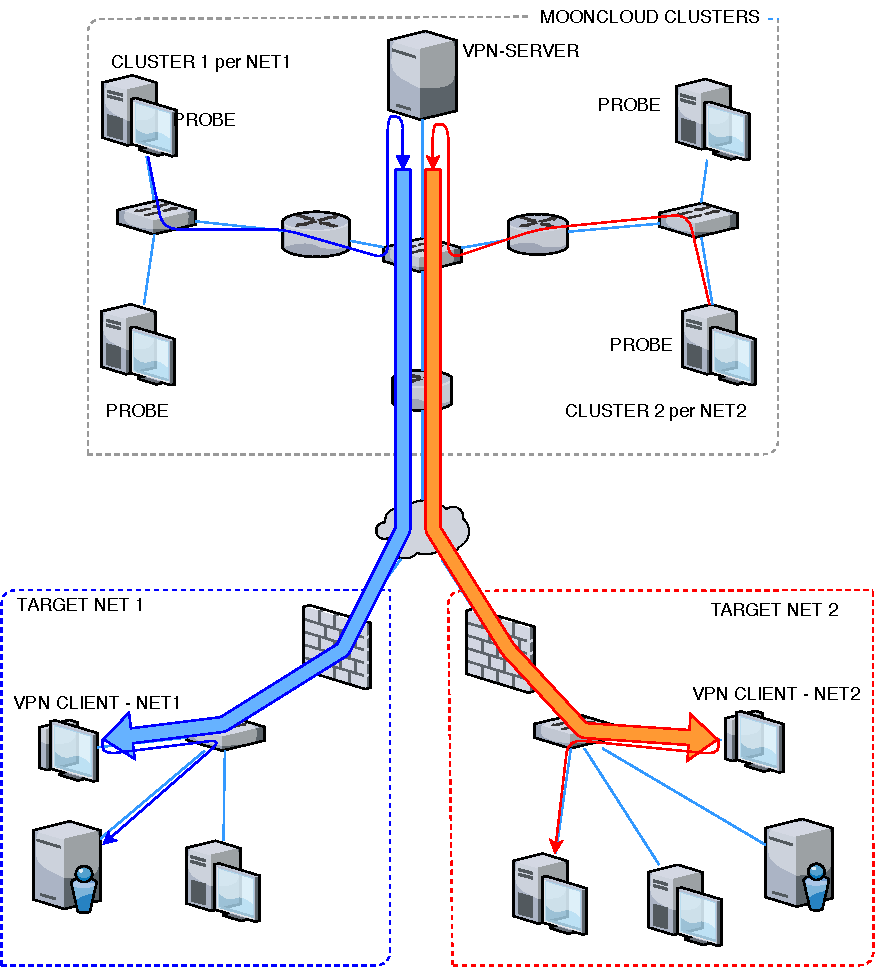
\includegraphics[scale=0.45]{img/ls}
	\end{figure}
\end{frame}


% \begin{frame}
%     \frametitle{MoonCloud\_VPN}
%     \alert{Microservizio} integrato in MoonCloud per gestire la soluzione VPN
%     \begin{itemize}
%         \item creazione file di \alert{configurazione} per \alert{OpenVPN}
%         \begin{itemize}
%             \item \alert{trasferimento} via SSH ai server
%         \end{itemize}
%         \item gestione \alert{certificati} di client e server
%         \begin{itemize}
%             \item creazione
%             \item revoca e rinnovo mediante \alert{CRL}
%         \end{itemize}
%         \item gestione \alert{IP mapping}
%         \begin{itemize}
%             \item assegnazione nuove reti ai client
%             \item creazione file di \alert{configurazione} per \alert{nftables}
%             \item dato un IP originale ritornare quello mappato
%         \end{itemize}
%     \end{itemize}
% \end{frame}


\begin{frame}
	\frametitle{NAT al contrario}
		
	\begin{itemize}
		\item IP src dei pacchetti MoonCloud verso la rete target
		      appartiene alla rete MoonCloud
		\item la rete target deve inviare le risposte al VPN client, ma senza
		      rotte configurate le invierebbe al proprio default gateway
	\end{itemize}
		
	\alert{NAT al contrario}: tutti i pacchetti provenienti dalla VPN vengono
	immessi nella rete target usando come IP sorgente quello del client VPN
	\begin{itemize}
		\item stesso NET ID della rete target
		\item quindi le risposte possono tornargli senza problemi
		\item realizzato con \alert{nftables}
	\end{itemize}
\end{frame}

\begin{frame}
	\frametitle{IP mapping}
	``\textit{Ogni rete connessa alla VPN deve stare in reti IP diverse}''\footnote{\url{https://openvpn.net}}
	\begin{itemize}
		\item si vuole che un server gestisca il maggior numero di reti target diverse
		\item alta probabilità che due reti abbiano lo stesso NET ID
	\end{itemize}
		
	\alert{IP mapping}: \textit{mappare} ogni rete target in una nuova rete
	\alert{garantita univoca} perché scelta da MoonCloud
	\begin{itemize}
		\item tutta MoonCloud conosce solo indirizzi mappati quindi unici
	\end{itemize}
\end{frame}

\begin{frame}
	\frametitle{IP mapping (2)}
	\begin{enumerate}
		\item Quando si registra un nuovo cliente, le sue reti vengono \alert{mappate}
		      in reti nuove ed univoche
		      		      
		\item il cliente specifica il target dell'analisi usando l'indirizzo IP reale
		      		              
		\item MoonCloud ne ottiene la \alert{versione mappata} in maniera tutto
		      \alert{trasparente}: è il l'IP dst dell'analisi
		      		      
		\item l'analisi parte, nel \alert{VPN client}
		      \begin{itemize}
		      	\item richieste MoonCloud $\rightarrow$ host target:
		      	      \begin{enumerate}
		      	      	\item modifica IP dst mappato $\rightarrow$ IP originale
		      	      	\item applica \textit{NAT al contario} ed invia ai target
		      	      \end{enumerate}
		      	\item risposte target $\rightarrow$ MoonCloud:
		      	      \begin{enumerate}
		      	      	\item applica inverso di \textit{NAT al contrario}
		      	      	\item modifica IP src originale $\rightarrow$ IP mappato
		      	      \end{enumerate}
		      \end{itemize}
		      		      
	\end{enumerate}
		
	\begin{itemize}
		\item per fare il mapping lato client si usa \alert{nftables}
	\end{itemize}
\end{frame}

\begin{frame}
	\frametitle{MoonCloud\_VPN}
	\alert{Microservizio} integrato in MoonCloud per gestire la soluzione VPN
	\begin{itemize}
		\item creazione file di \alert{configurazione} per \alert{OpenVPN}
		      \begin{itemize}
		      	\item \alert{trasferimento} via SSH ai server
		      \end{itemize}
		\item gestione \alert{certificati} di client e server
		      \begin{itemize}
		      	\item creazione
		      	\item revoca e rinnovo mediante \alert{CRL}
		      \end{itemize}
		\item gestione \alert{IP mapping}
		      \begin{itemize}
		      	\item assegnazione nuove reti ai client
		      	\item creazione file di \alert{configurazione} per \alert{nftables}
		      	\item dato un IP originale ritornare quello mappato
		      \end{itemize}
	\end{itemize}
\end{frame}

\begin{frame}
	\frametitle{Sicurezza}
	Il device VPN viene portato in una rete \alert{non trusted} quindi
	occorre \alert{proteggere MoonCloud}:
	\begin{itemize}
		\item \alert{regole di firewalling} sui VPN server che consentano
		      alle \alert{sole richieste e risposte} da/per MoonCloud di transitare
	\end{itemize}
	
	\begin{itemize}
		\item si utilizza ancora \alert{nftables}
	\end{itemize}
\end{frame}

